\chapter{Efekt działania}
\label{cha:efekt}



%----------------------------------------------------------------------------------------
% Rozbudować
% - tu są tylko główne myśli
% - 
%----------------------------------------------------------------------------------------
\section{Efekt działania}
W tym rozdziale zostały zebrane zdjęcia zrobione podczas testowania algorytmu. Niestety z powodu braku odpowiedniego sprzętu zdjęcia te zostały zrobione w słabej jakości. Warto zauważyć, że w bazie znajdowały się również wartości RGB dla ludzi o różnej karnacji. Skutkuje to tym, iż na zdjęciu \ref{fig:5} sieć bez problemu rozpoznaje również skórę innej karnacji.\\ \\ 
\begin{figure}[tbph!]
\centering
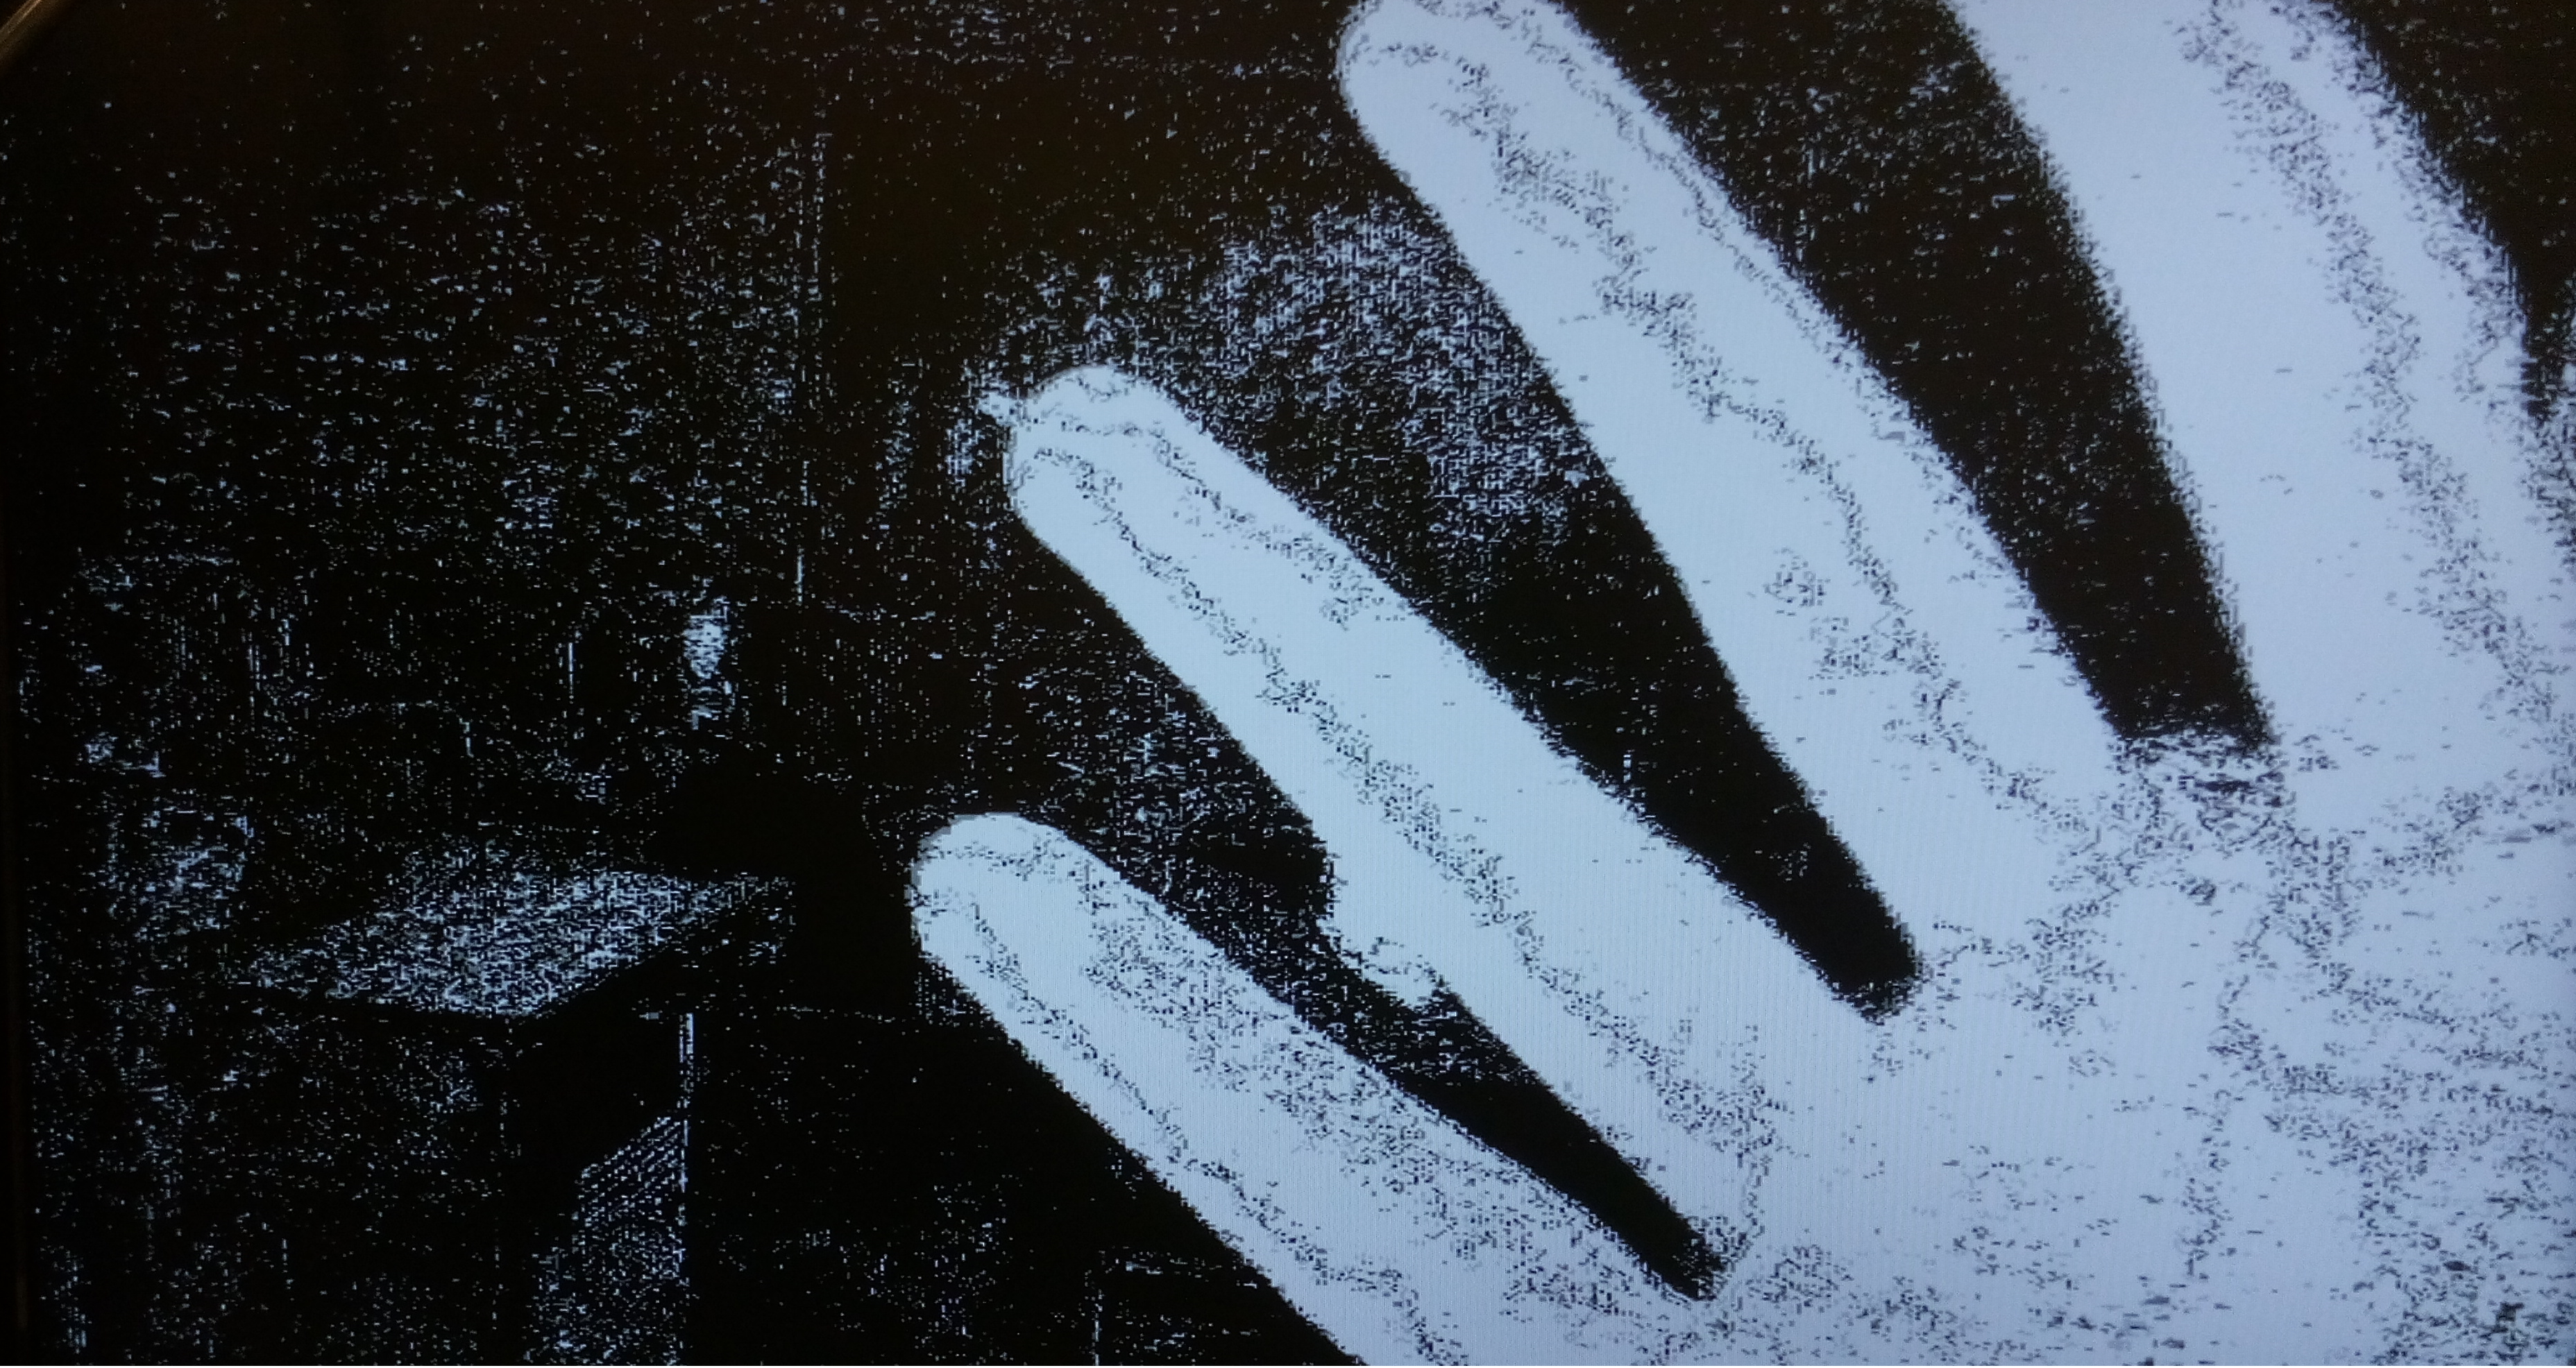
\includegraphics[width=0.9\linewidth]{images/1.png}
\caption{Struktura katalogów}
\label{fig:1}
\end{figure}
\begin{figure}[tbph!]
\centering
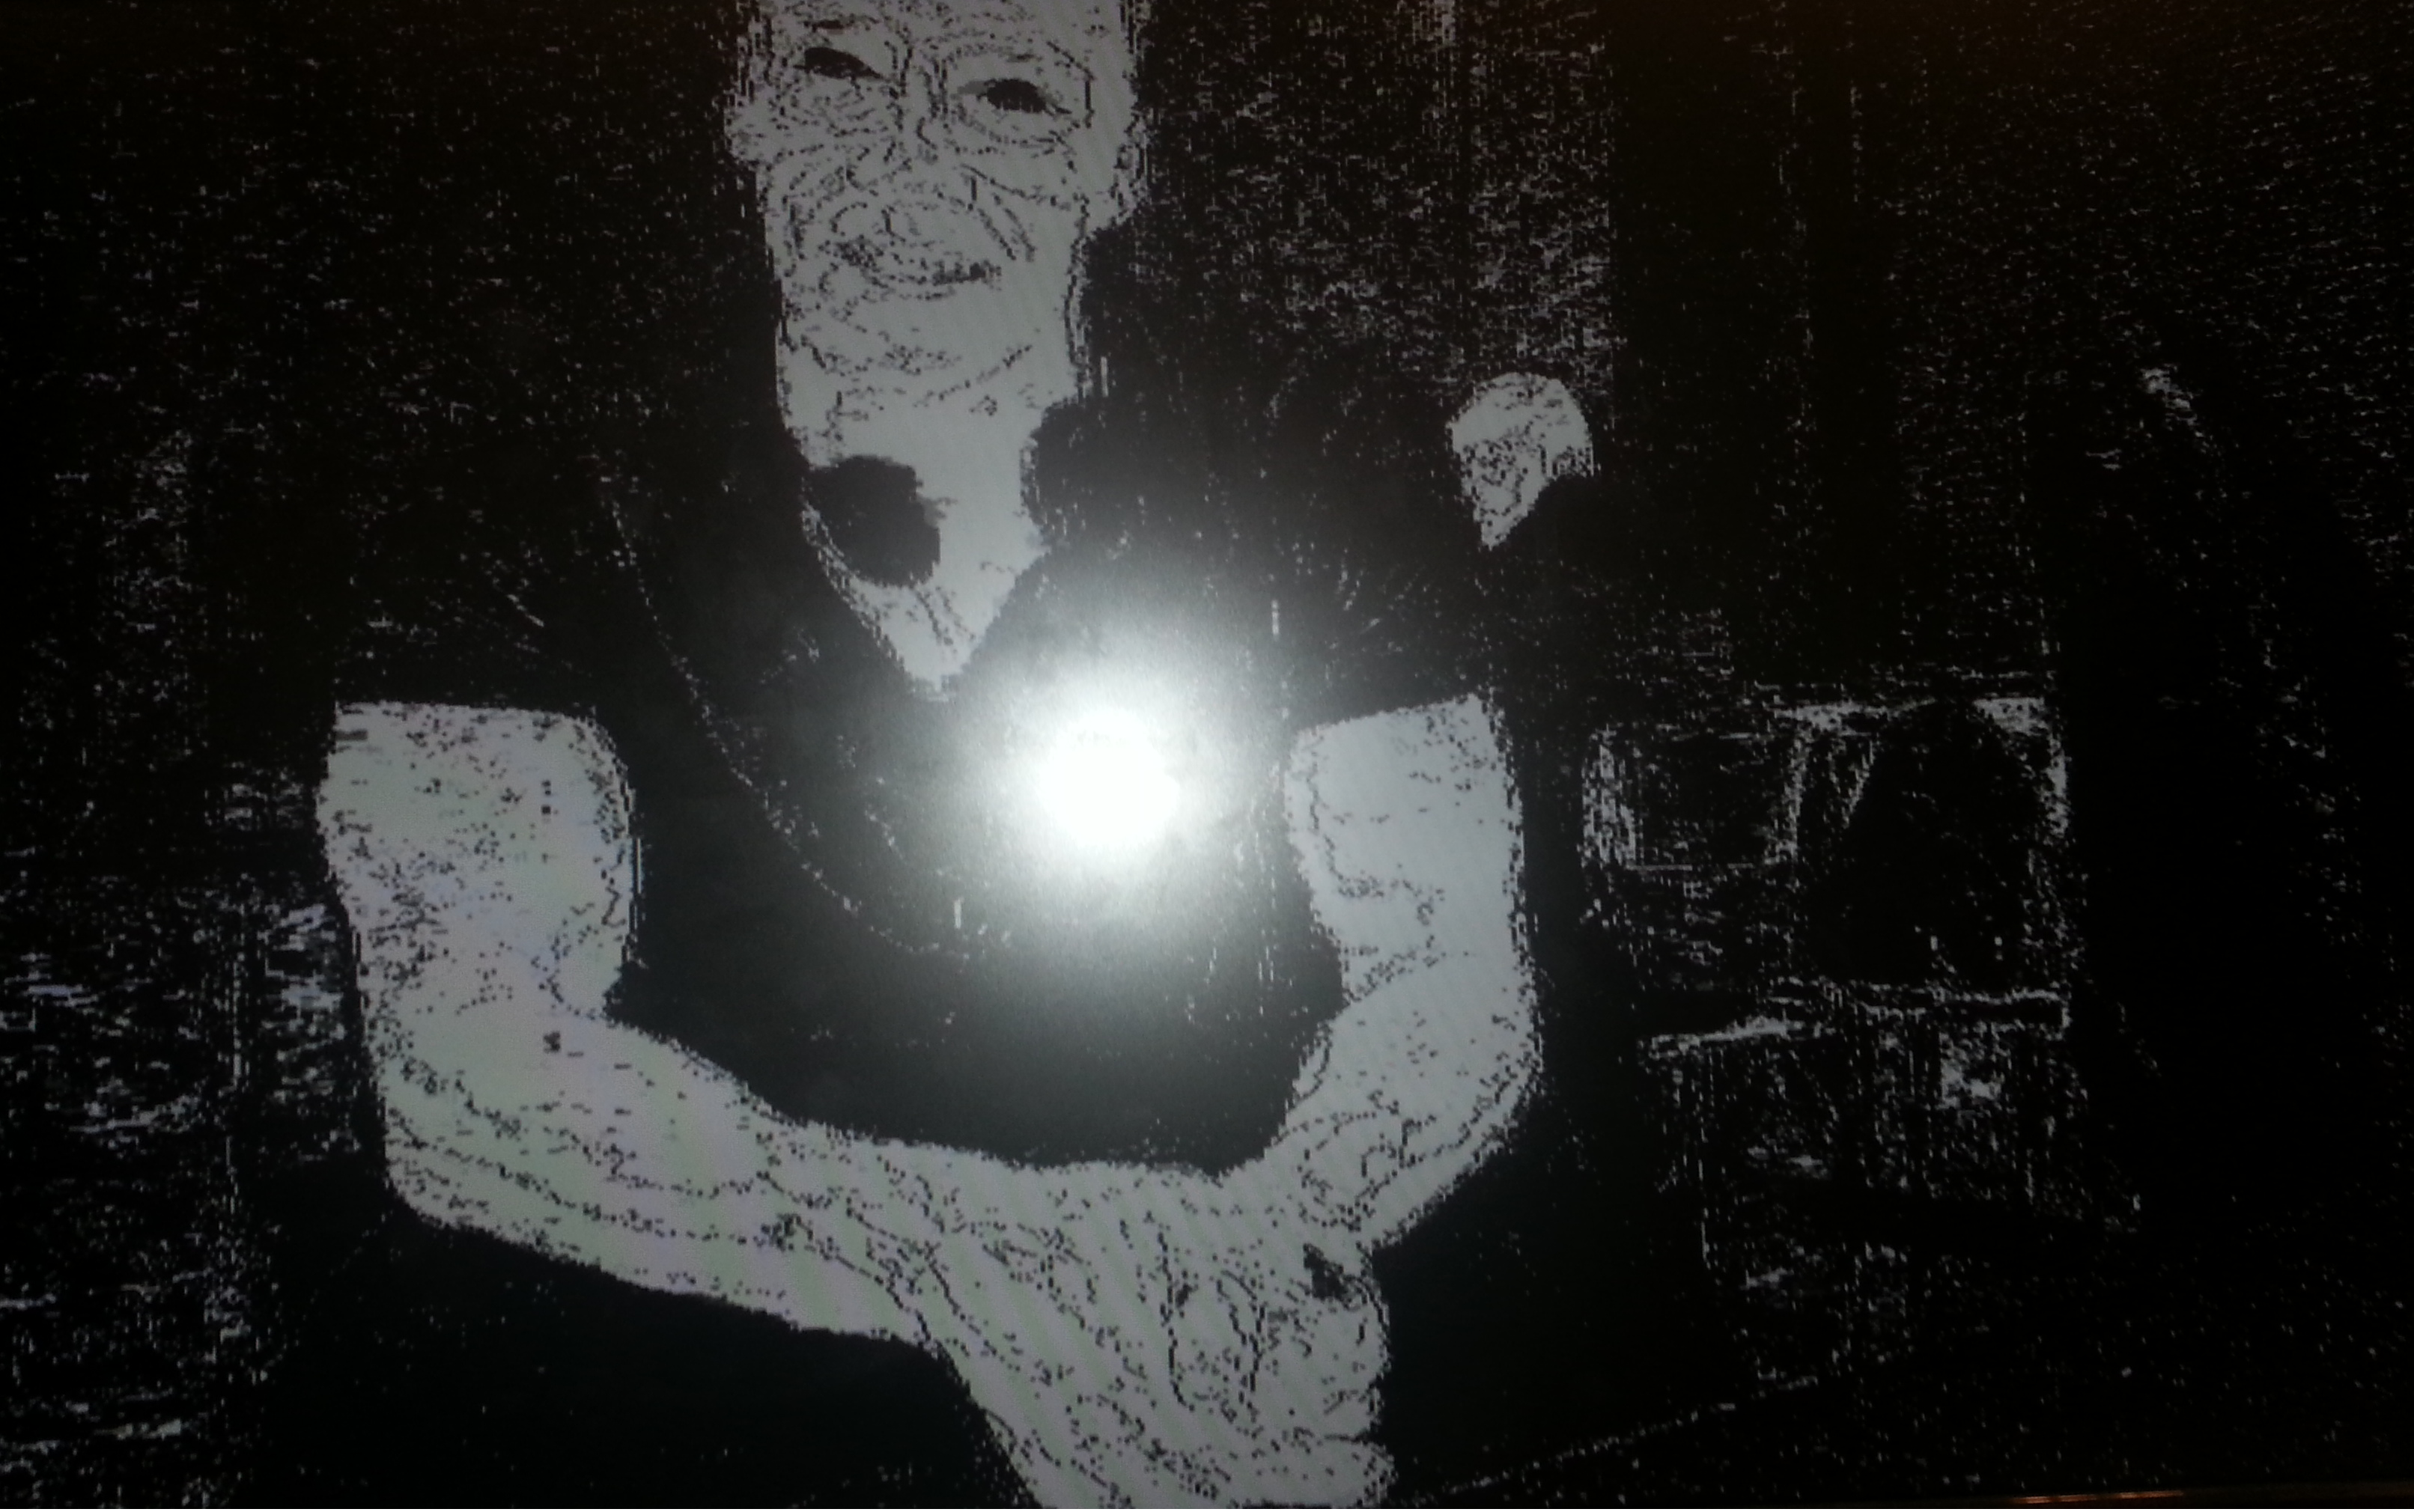
\includegraphics[width=0.9\linewidth]{images/3.png}
\caption{Struktura katalogów}
\label{fig:2}
\end{figure}
\begin{figure}[tbph!]
\centering
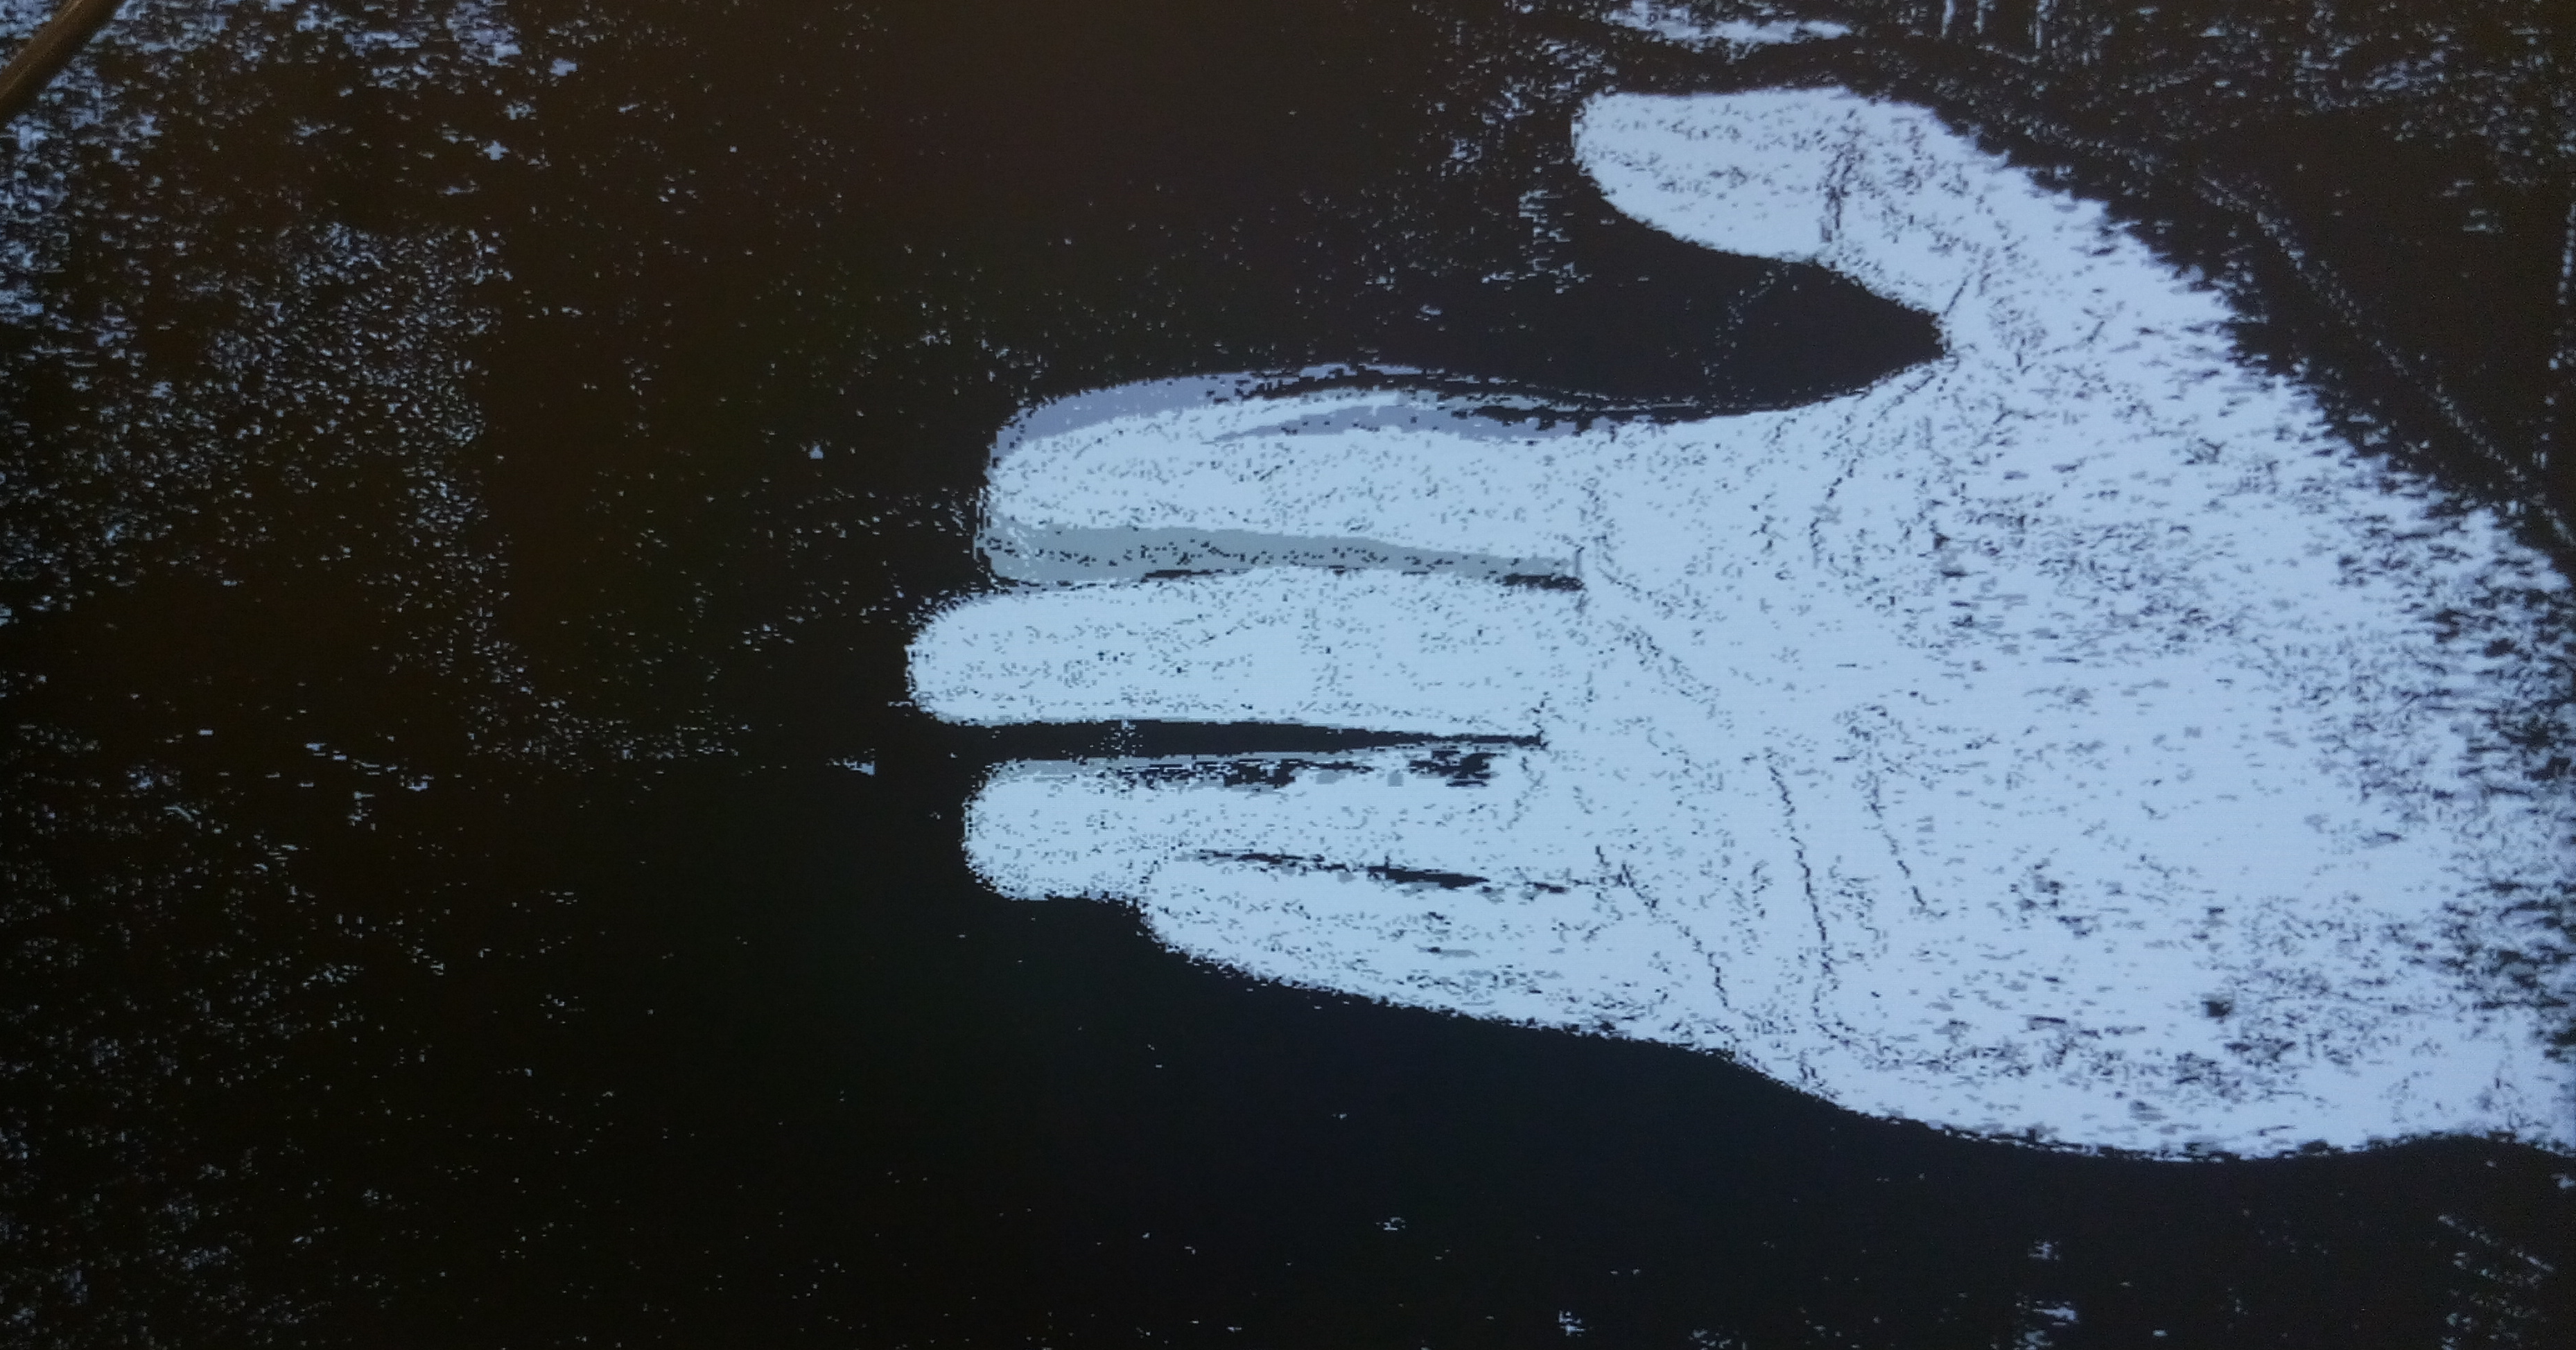
\includegraphics[width=0.9\linewidth]{images/2.png}
\caption{Struktura katalogów}
\label{fig:3}
\end{figure}
\begin{figure}[tbph!]
\centering
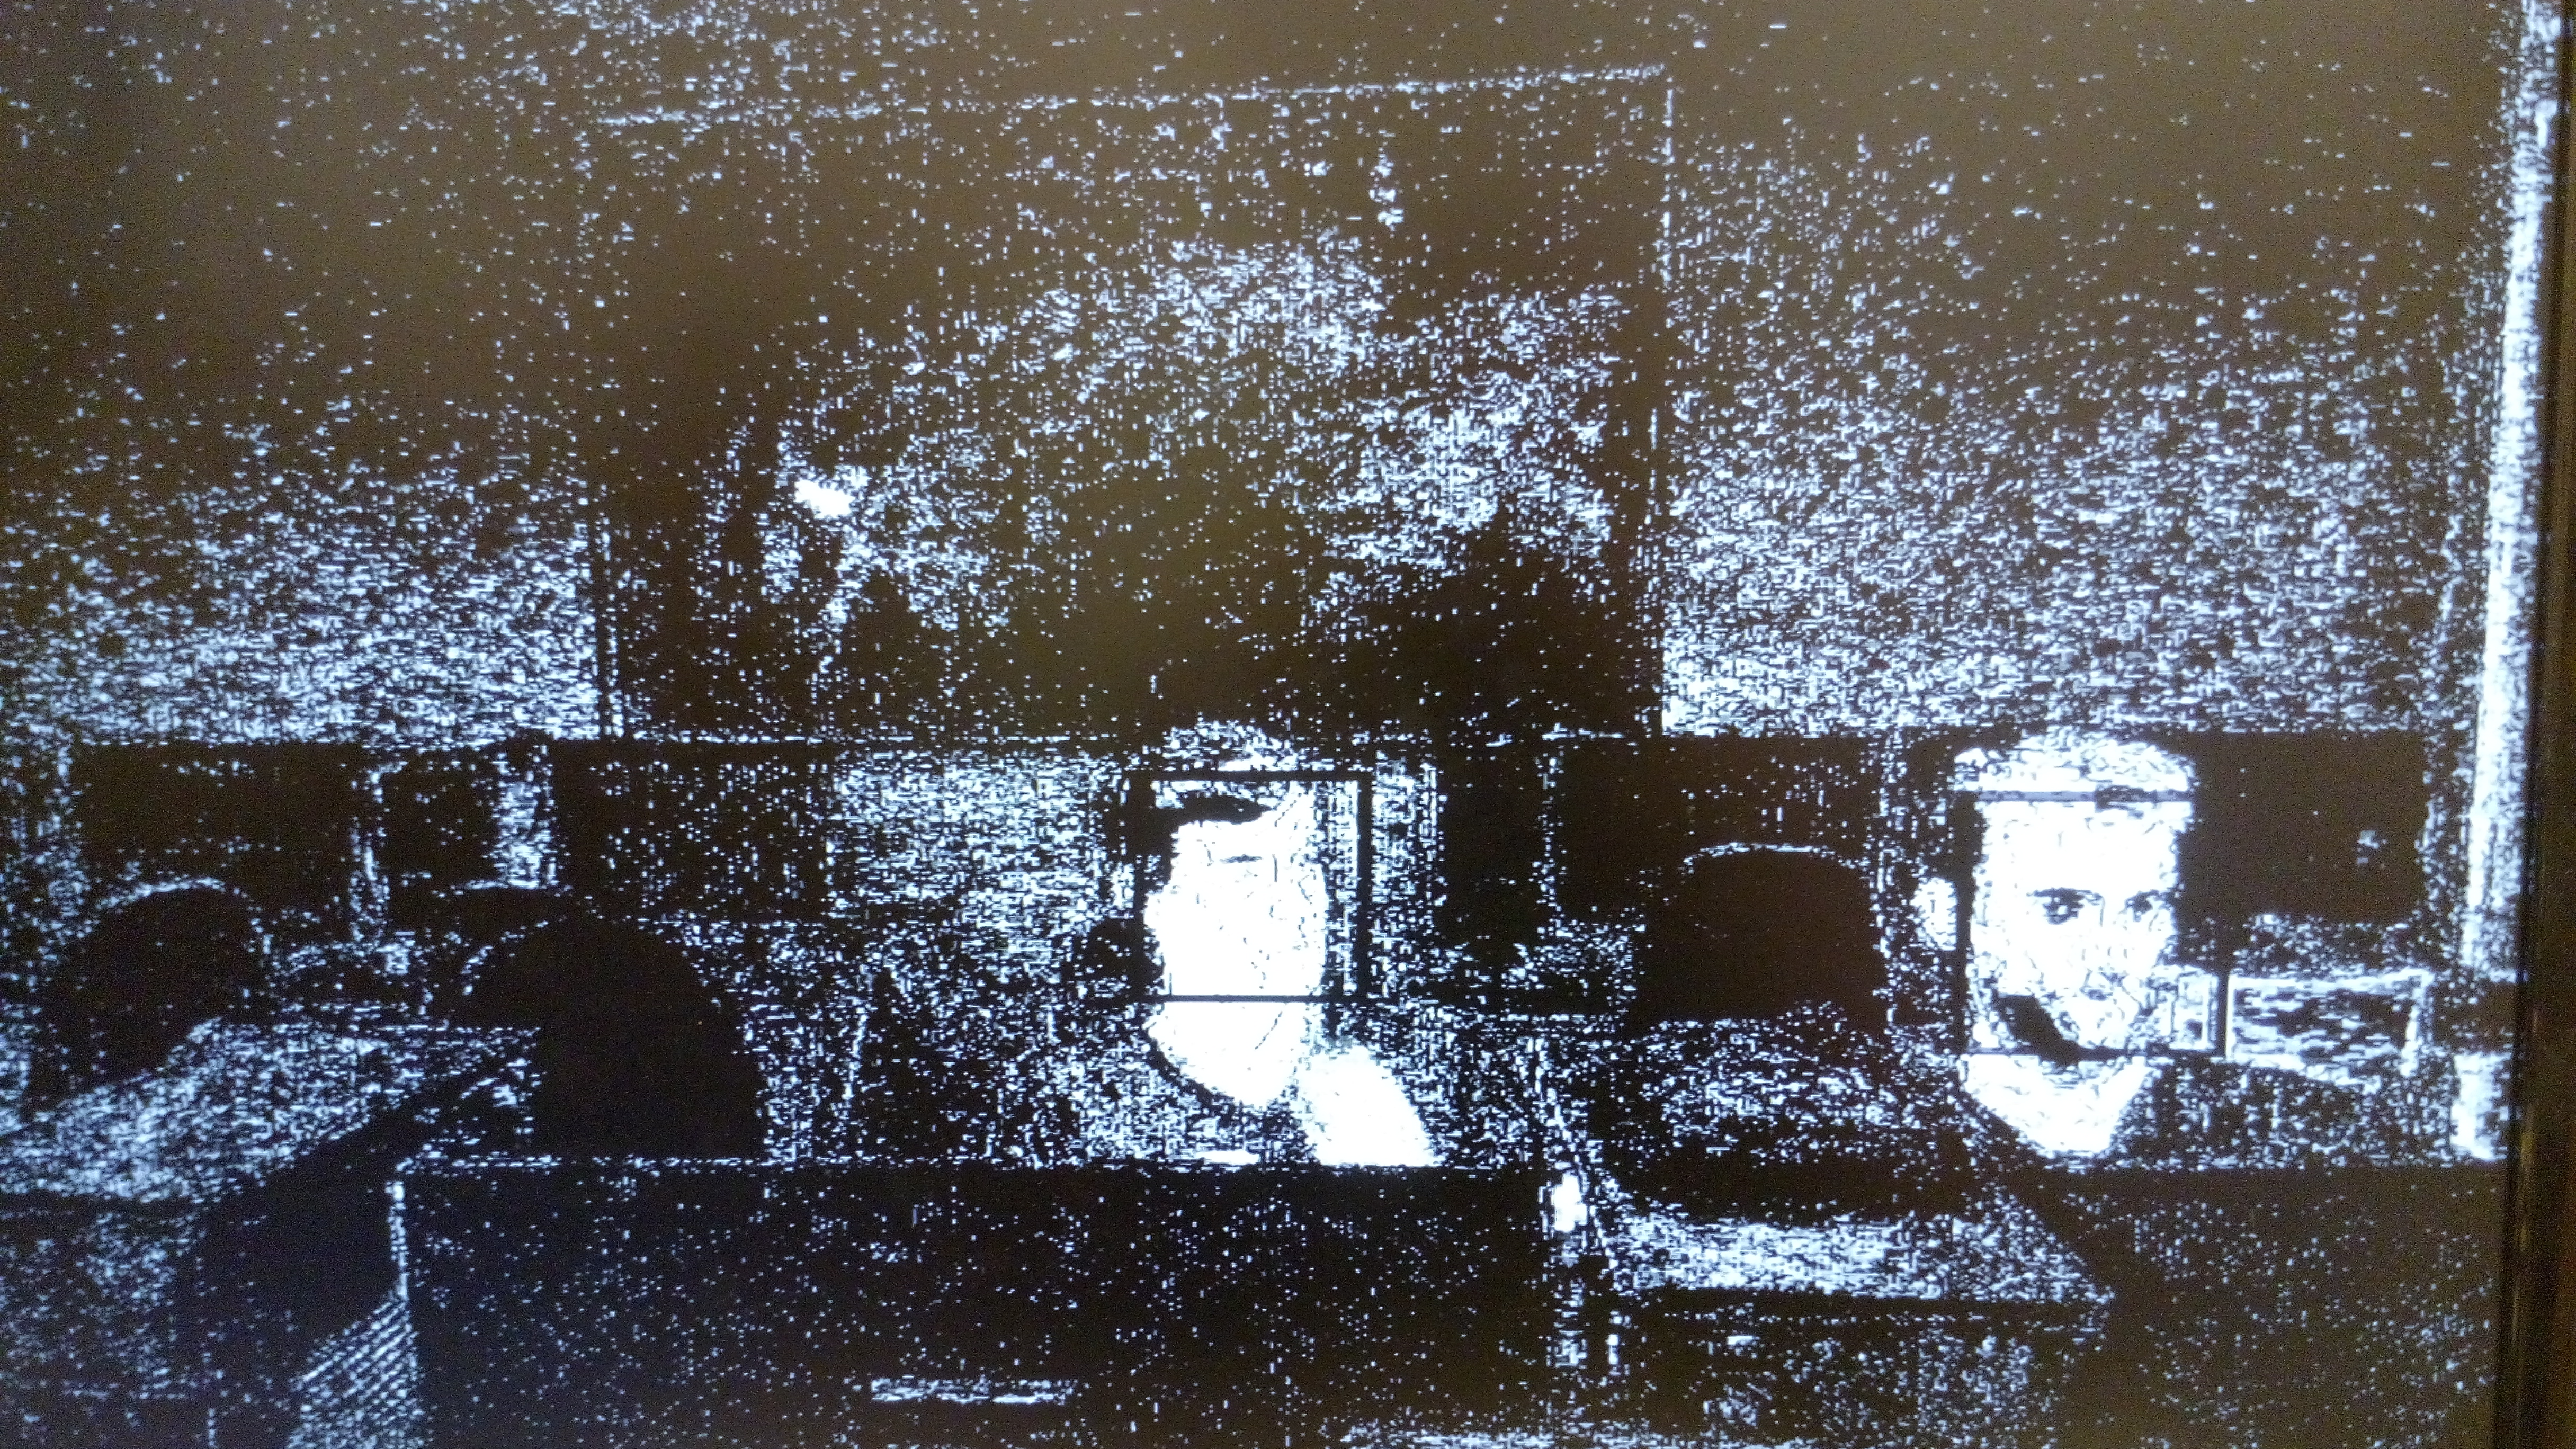
\includegraphics[width=0.9\linewidth]{images/5.png}
\caption{Struktura katalogów}
\label{fig:4}
\end{figure}
\begin{figure}[tbph!]
\centering
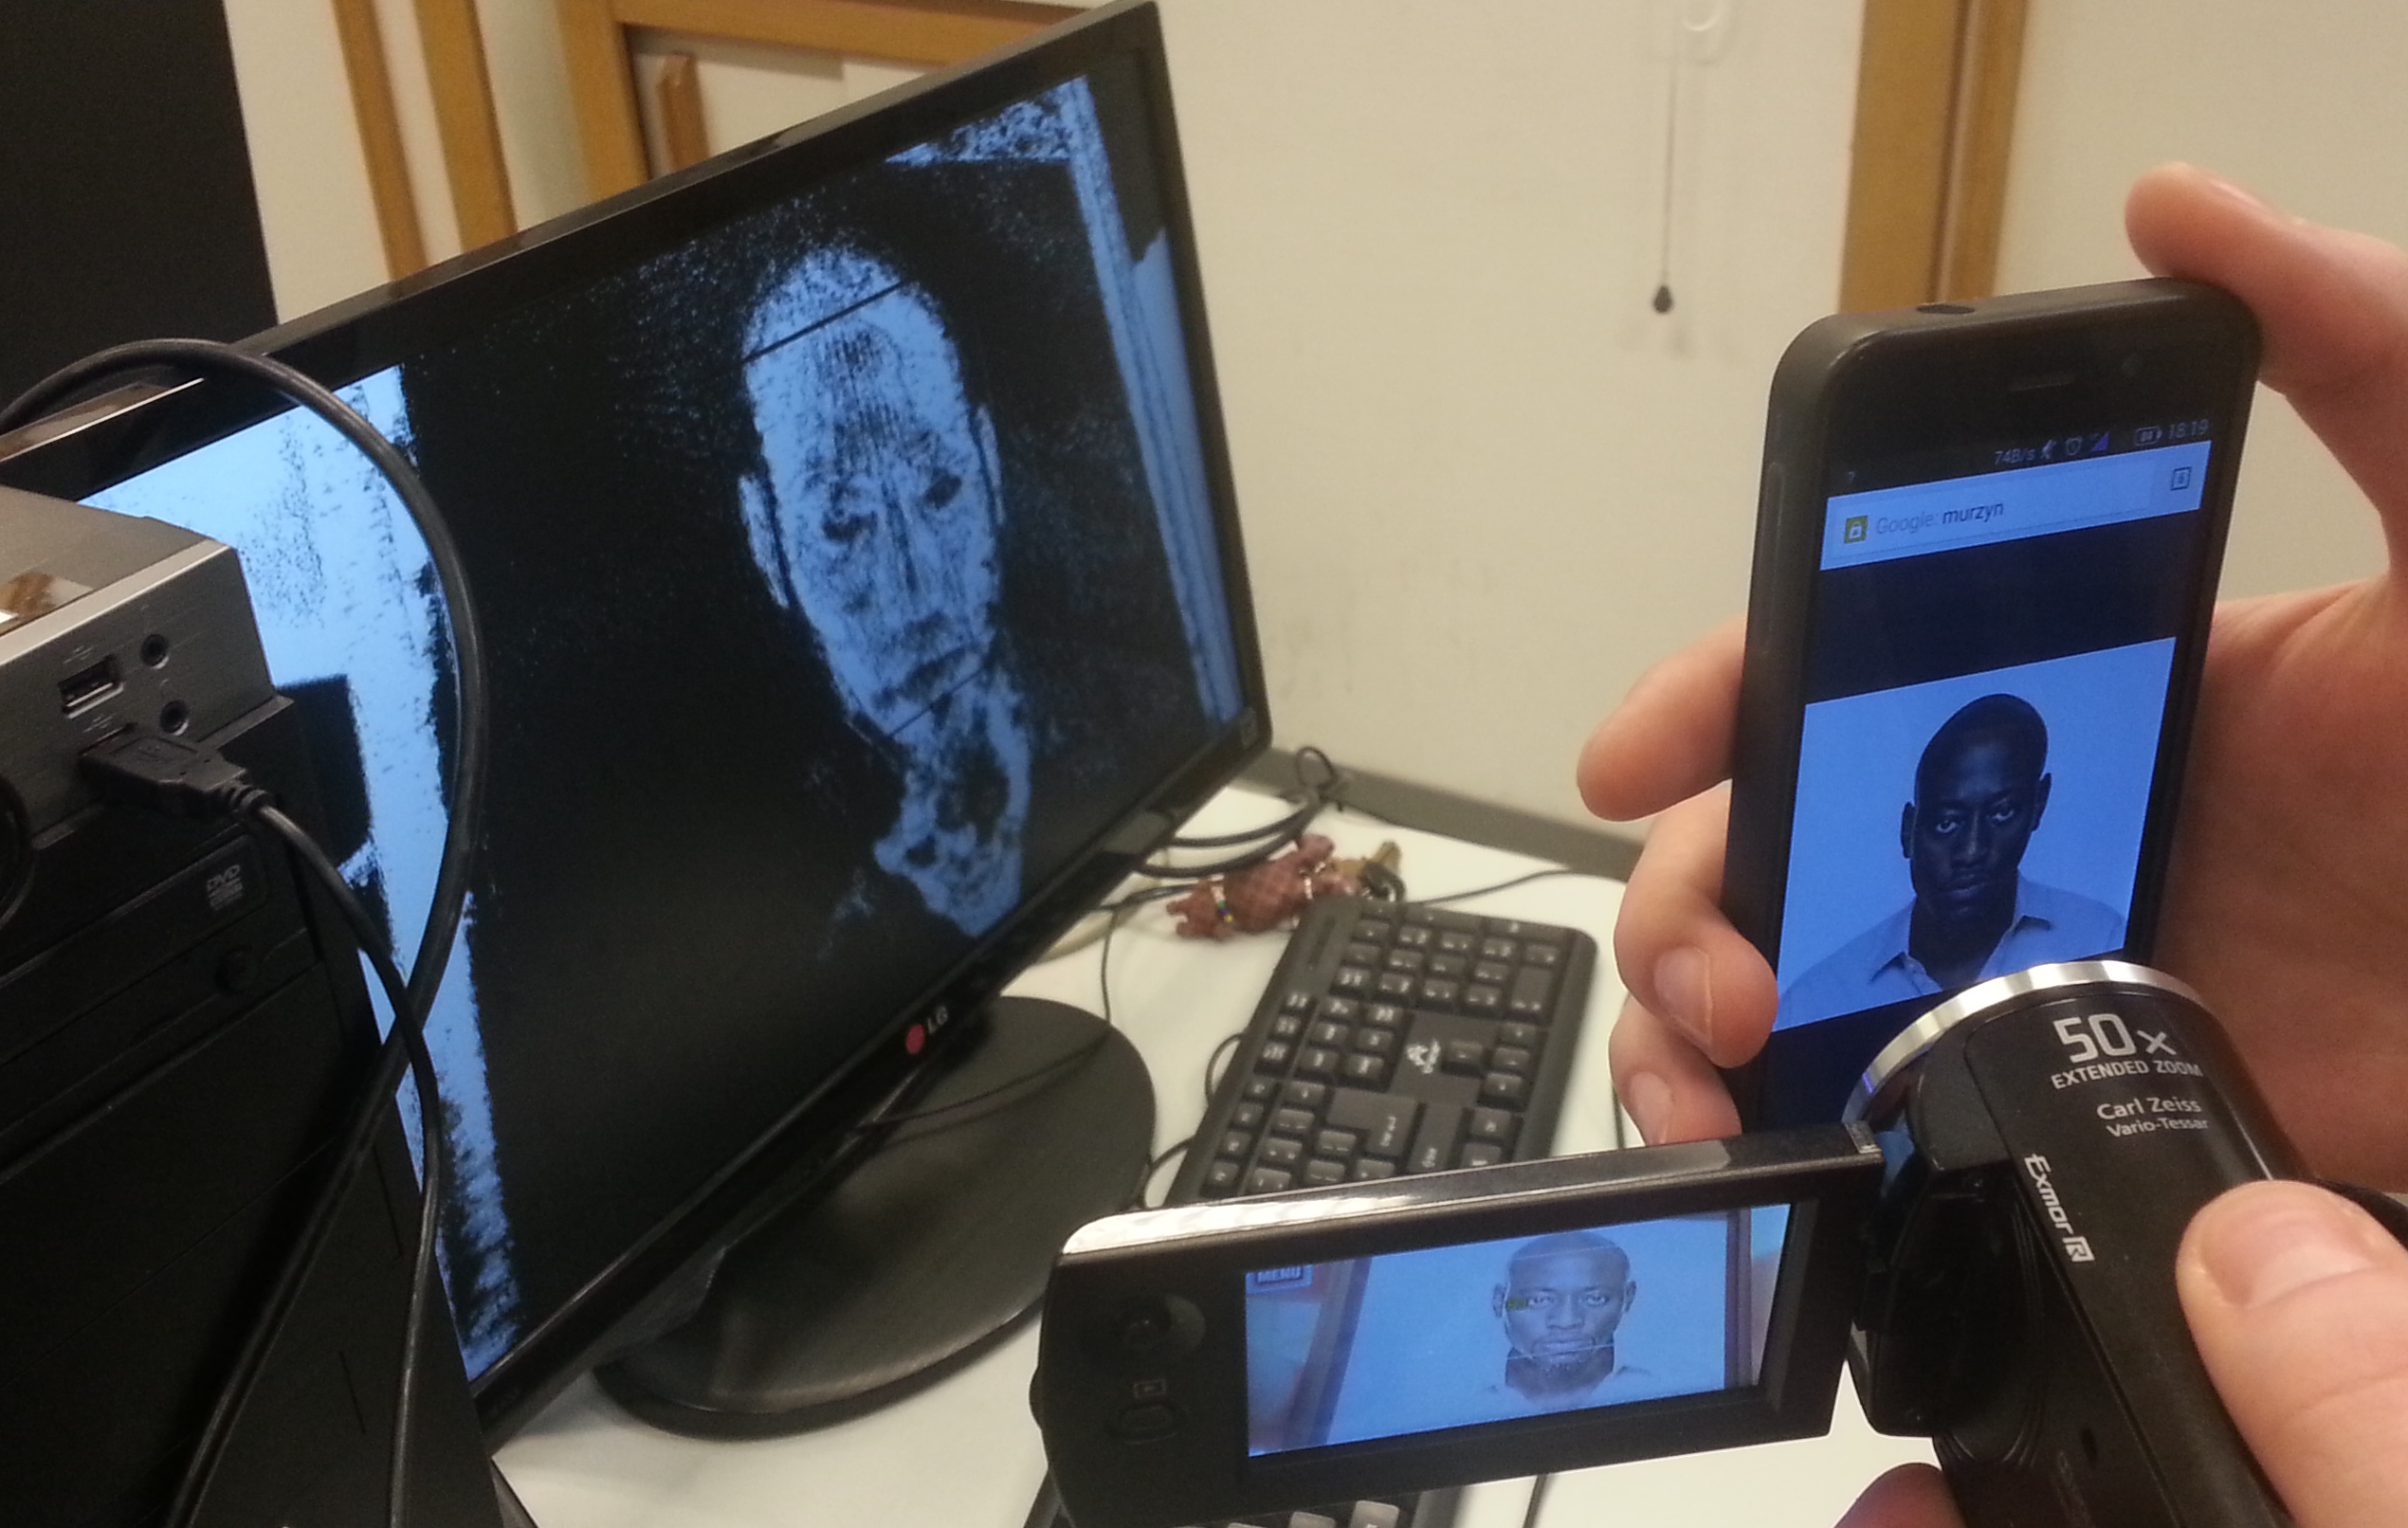
\includegraphics[width=0.9\linewidth]{images/4.png}
\caption{Struktura katalogów}
\label{fig:5}
\end{figure}
